%%%%%%%%%%%%%%%%%%%%%%%%%%%%%%%%%%%%%%%%%
% Stylish Article
% LaTeX Template
% Version 2.1 (1/10/15)
%
% This template has been downloaded from:
% http://www.LaTeXTemplates.com
%
% Original author:
% Mathias Legrand (legrand.mathias@gmail.com) 
% With extensive modifications by:
% Vel (vel@latextemplates.com)
%
% License:
% CC BY-NC-SA 3.0 (http://creativecommons.org/licenses/by-nc-sa/3.0/)
%
%%%%%%%%%%%%%%%%%%%%%%%%%%%%%%%%%%%%%%%%%

%-------------------------------------------------------------------------------------
%	PACKAGES 
%-------------------------------------------------------------------------------------

\documentclass[fleqn,11pt]{SelfArx} % Document font size and equations flushed left
\usepackage[francais]{babel} % Specify a different language here - english by default
\usepackage{hyperref}

\setlength{\columnsep}{0.55cm} % Distance between the two columns of text
\setlength{\fboxrule}{0.75pt} % Width of the border around the abstract
\definecolor{color1}{RGB}{0,0,90} % Color of the article title and sections
\definecolor{color2}{RGB}{0,20,20} % Color of the boxes behind the abstract and headings
\usepackage{hyperref} % Required for hyperlinks
\usepackage{xcolor}  
\usepackage{listings}
\usepackage{pdfpages}
\usepackage{amssymb}
%\usepackage[french]{babel}

\usepackage{courier} % Required for the courier font         
\hypersetup{hidelinks,colorlinks,breaklinks=true,urlcolor=blue,citecolor=color1,linkcolor=color1, bookmarksopen=false,pdftitle={Title},pdfauthor={Author}}

\providecommand\phantomsection{}


%--------------------------------------------------------------------------------------
%	CODE INCLUSION CONFIGURATION
%-------------------------------------------------------------------------------------
\usepackage{color}
 
\definecolor{codegreen}{rgb}{0,0.6,0}
\definecolor{codegray}{rgb}{0.5,0.5,0.5}
\definecolor{codepurple}{rgb}{0.58,0,0.82}
\definecolor{backcolour}{rgb}{0.95,0.95,0.92}
 
\lstdefinestyle{mystyle}{
    backgroundcolor=\color{backcolour},   
    commentstyle=\color{codegreen},
    keywordstyle=\color{magenta},
    numberstyle=\tiny\color{codegray},
    stringstyle=\color{codepurple},
    basicstyle=\footnotesize,
    breakatwhitespace=false,         
    breaklines=true,                 
    captionpos=b,                    
    keepspaces=true,                 
    numbers=left,                    
    numbersep=5pt,                  
    showspaces=false,                
    showstringspaces=false,
    showtabs=false,                  
    tabsize=2
}
 
\lstset{style=mystyle}



%-------------------------------------------------------------------------------------
%	INFORMATIONS
%-------------------------------------------------------------------------------------


\JournalInfo{Projet RESYS 2016-2017}
\Archive{Master 2 BIM-BMC, UPMC} 
\PaperTitle{Différenciation des précurseurs hématopoïétiques chez l'embryon}
\Authors{Nathalie Lehmann\textsuperscript{1}, Mariam Sissoko\textsuperscript{1} \\ Enseignants référents: \textbf{Hervé Isambert\textsuperscript{2}, Louis Verny\textsuperscript{2}, Nadir Sella\textsuperscript{2}}}

\affiliation{\textsuperscript{1}\textit{Master 2 Bioinformatique et Modélisation, Université Paris 6, France}}
\affiliation{\textsuperscript{2}\textit{Institut Curie, France}}


\Keywords{Réseaux de régulation -- Facteurs de transcription -- Hématopoïèse} 

\newcommand{\keywordname}{Mots-clés} %--------------------------------------------------------------------------------------
%	ABSTRACT
%--------------------------------------------------------------------------------------

\Abstract{Le but de ce projet de Master 2 de bioinformatique est de reconstruire le réseau de régulation régissant les expressions des facteurs de transcription clés pour la différenciation des précurseurs hématopoïétiques chez l'embryon. Dans cet objectif, nous avons d'abord procédé à un filtrage des données afin de garder les gènes d'intérêt, puis reconstruit des réseaux selon deux méthodes différentes : par clustering hierarchique et via l'algorithme polynomial PC\cite{pc} (\textit{Peter-Clark}). Enfin, en comparant nos résultats avec ceux présents dans la littérature scientifique, nous avons fait état d'un modèle graphique simplifié expliquant les mécanismes impliquant la différenciation des cellules primitives en deux lignées distinctes : hématopoïétique et endothéliale. Ainsi, nous avons pu visualiser le rôle central de certains facteurs de transcription (FT), dont Tal1, l'\textit{erythroid differentiation factor} connu pour son implication dans différents cas de leucémies, ou Runx1 pour induire les précurseurs des cellules épithéliales. Cette reconstruction de réseau a été effectuée à partir de données analysées par \textit{single cell RNA-seq} puis binarisées. }


%--------------------------DEBUT-------------------------------------

\begin{document}
\flushbottom 
\maketitle


\tableofcontents 

\thispagestyle{empty} 


%------------------------------------------------
%--------------INTRO----------------------------------
%------------------------------------------------
\section*{Introduction}
\addcontentsline{toc}{section}{Introduction}
Au cours du développement de l'embryon des Verté-brés, tous les tissus hématopoïétiques successivement actifs (foie, thymus, rate et moelle osseuse) sont colonisés par des cellules souches hématopoïétiques (CSH) d'origine extrinsèque. Le sac vitellin (SV) constitue l'unique exception à cette règle, puisque des CSH s'y développent in situ. Il a été observé que le SV constitue le premier site d'hématopoïèse de l'embryon\cite{Cumano} : c'est le lieu d'apparition des premières cellules sanguines propres à l'embryon. Cependant, de la lignée primitive à l'origine de celles-ci, émerge aussi les premières cellules endothéliales (constituant la paroi interne des vaisseaux sanguins). Dans ces conditions, quels sont les facteurs de transcription suffisants et/ou nécéssaires pour induire cette différenciation de la lignée primitive ?

\par Reconstruire le réseau de régulation contôlant cette différenciation pourrait permet de mieux appréhender les mécanismes de l'hématopoïèse primitive et de la formation des tissus sanguins. Or l'origine de certaines leucémies (ie l'anémie de Fanconi\cite{Fanconi}) reste encore difficile à déterminer, et l'établissement de tels réseaux pourrait alors favoriser la compréhension et l'établissement de protocoles expérimentaux mieux ciblés. 
 
\par Il est important de spécifier que ce projet s'appuie largement sur l'article de Moignard et al., \textit{Decoding the regulatory network of early blood development from single-cell expression measurements}\cite{Moignard}. En effet, les données utilisées pour réaliser ce projet sont similaires à celles utilisées par les auteurs de l'article sus-nommé, et la démarche globale de reconstruction de réseau est relativement semblable, bien qu'allégrement simplifiée. 


%------------------------------------------------
%--------------METHODES----------------------------------
%------------------------------------------------

\section{Données et méthodes}
La reconstruction des voies moléculaires contrôlant le développement embryonique des organes est entrâvé par le manque de méthodes adaptées pour l'étude de phénomènes extrêmement précis, d'autant plus si le matériel disponible est limitant. Les techniques traditionnelles telles que le RNA-seq se révèlent alors insuffisantes. La stratégie que les auteurs de l'article de référence ont choisi est particulièrement pertinente car il s'agit d'une approche combinant le séquençage \textit{single cell} et les analyses computationnelles de reconstruction de réseaux à partir des graphes des états de transition. En effet, le séquençage \textit{single cell} (sc) permet une analyse transcriptomique à l'échelle d'une seule cellule. Grâce au sc-RNAseq, il devient possible d'estimer l'hétérogénéité intra-tumorale, mais aussi d'étudier des stades embryonnaires précoces, ou encore de retracer les lignées cellulaires au cours du développement (source : \href{http://bioinfo-fr.net/single-cell-sequencing?hilite=single+cell+RNA-seq}{bioinfo-fr} )\footnote{http://bioinfo-fr.net}. 


\subsection{Dataset}
Le dataset proposé rassemble les données d'expression binarisées de différents gènes pouvant soit être des facteurs de transcription (33 gènes), soit d'autres gènes marqueurs (spatiaux ou temporels - 9 gènes), ou encore des gènes servant de contrôle (\textit{housekeepers} - 4 gènes). Chaque ligne du dataset correspond au profil d'expression d'une cellule, analysée par sc-RNAseq. Les colonnes, quant à elles, correspondent aux gènes dont l'expression a été quantifiée. Les données étant binaires, le '1' représente un gène exprimé dans la condition correspondante, le '0' un gène non exprimé. Au total, cela fait donc 46 gènes analysés dans 3934 cellules issues d’embryons de souris, prelevées à quatre stades différents du développement embryonnaire précoce. Celles-ci deviendront éventuellement des cellules sanguines (en rouge sur la figure \ref{fig:debut}) ou endothéliales (en violet). Comme indiqué sur la figure \ref{fig:debut}, cinq populations sont analysées :

\begin{itemize}
\item E7.0 (\textit{primitive streak}, PS),
\item E7.5 (\textit{neural plate}, NP) 
\item E7.75 (\textit{head fold}, HF).
\item E8.25, cellules GFP+ (\textit{four somite}, 4SG) cellules sanguines potentielles
\item E8.25, cellules Flk1+GFP− (4SFG−) cellules endothéliales potentielles.
\end{itemize}



\begin{figure}[ht]
\centering
\includegraphics[width=\linewidth]{images/debut2}
\caption{Processus de différenciation de la lignée primitive (PS) en 2 lignées distinctes : endothéliale (4SFG) et hématopoïétique (4SG)}
\label{fig:debut}
\end{figure}

Les étapes critiques du développement hématopoïétique murin sont recensées figure \ref{fig:devpt} en annexe.



\subsection{Filtre des données}
Afin d'obtenir un set de données non biaisées, nous avons choisi d'appliquer un filtre afin d'éliminer les gènes exprimés dans 100\% des cas (codé en Python, on ôte du dataset les colonnes où il n'existe que des '1'). Les gènes qui disparaissent alors sont référencés, et leur fonction en tant que \textit{housekeepers} a été vérifiée via le site de la \href{https://www.ncbi.nlm.nih.gov/gene}{NCBI}\footnote{https://www.ncbi.nlm.nih.gov/gene} ou via le site \href{http://www.genecards.org/}{Gene Cards}\footnote{Dans toute la suite du document, les fonctions des gènes ont été identifiées via le site Gene Cards.}: \textbf{Eif2b1}, \textbf{Mrpl19}, \textbf{Polr2a}, \textbf{Ubc}.

%/ ou via mouse genom database

\begin{figure*}[ht]
\centering
\includegraphics[width=\linewidth]{images/pc}
\caption{Algorithme PC (Spirtes, Glymour, Scheines (1993)}
\label{fig:pc}
\end{figure*}

\subsection{Gènes d'intérêt}

Une fois le filtre appliqué, il nous a fallu procéder à différents tris des données. 
\subsubsection{Tri par facteur de transcription}
Les 42 gènes restant dans notre dataset n'étant pas tous impliqués directement dans la différenciation cellulaire, nous avons effectué un premier tri où ne sont conservés que les 33 facteurs de transcription. Les gènes marqueurs qui ne se trouvent plus dans le dataset codent pour les protéines suivantes : les protéines d'adhésion cellulaire calcio-dépendantes \textbf{Cdh1} et \textbf{Cdh5}, une sous-unité du facteur d'initiation de la traduction 
\textbf{EgfI7}, la globine embryonnaire \textbf{Hbb-bH1}, les récepteurs \textbf{Itga2b} (ou CD41), \textbf{Kit}, \textbf{Procr} et \textbf{Kdr} (ce dernier étant un récepteur de la VEGF - \textit{Vascular endothelial growth factor}), et enfin \textbf{Pecam1}, une protéine de surface impliquée dans les jonctions inter-cellulaires des cellules endothéliales. En fonction de leur rôle et de leur localisation, certains de ces gènes jouent un rôle clé pour la différenciation des précurseurs hématopoïétiques, et cela peut être facilement visualisé sur les réseaux qui ont été reconstruits. Ainsi, dans chacun des tris décrits ci-dessous, a été conservé un dataset avec les 42 gènes, et un autre avec les 33 facteurs de transciption afin de permettre d'analyser de façon spécifique toutes les interactions potentielles.
\subsubsection{Tri par stade embryonnaire}
Afin d'étudier les relations au niveau temporel, les données ont été séparées par type cellulaire présent dans le dataset (PS, NP, HF, 4SFG, 4SG). 
\subsubsection{Tri par lignée}
Enfin, une séparation des données au niveau fonctionnel a été effectué. Nous avons alors un dataset pour les gènes préférentiellement exprimés dans la lignée primitive (en bleu sur la figure \ref{fig:filtre33prof}), un autre dont les gènes sont davantage associés à l'hématopoïèse (en rouge) et le dernier pour les gènes impliqués dans la formation de l'endothélium (en rose/violet).


\subsection{Reconstruction de réseaux}
Un réseau est défini comme un ensemble de points appelés noeuds connectés entre-eux par des liens, ces derniers pouvant être orientés ou non. On appelle degré d'un noeud le nombre de liens que celui-ci établi avec ses voisins. Dans le cas d'un réseau orienté, le degré regroupe les liens entrants et sortants. Dans notre étude, les réseaux ont été établis en définissant les gènes pour noeuds et les interactions de régulation (activation ou inhibition) comme liens (les données étant des niveaux d'expression binarisés comme décrit ci-dessus). Nous avons choisi d'utiliser deux types d'algorithmes différents.

\begin{figure*}[ht]
\centering
\includegraphics[width=\linewidth]{results/arbre33genes}
\caption{Arbre obtenu par clustering hierarchique non supervisé - 33 gènes}
\label{fig:arbre33}
\end{figure*}

\subsubsection{Algorithme PC}
Une première démarche pour reconstruire les réseaux est d'appliquer l'algorithme PC\cite{pc} (Peter-Clark). Il s'agit d'un algorithme polynomial pour l'inférence de l'architecture des réseaux. Pour cela, deux choix s'offraient à nous : utiliser le package \textit{pcalg} disponible sur R, ou bien le \href{https://miic.curie.fr}{Miic Web Server}\footnote{https://miic.curie.fr} (\textit{Multivariate Information based Inductive Causation}), outil développé par l'équipe enseignante. La robustesse de l'outil, la maîtrise facile de l'interface et la diversité des paramètres modifiables pour la manipulation des données ont vite orienté notre choix pour l'utilisation de ce dernier. Nous avons notamment fait usage de l'interface \href{http://cytoscape.org}{Cytoscape}\footnote{http://cytoscape.org} accessible via le Miic Web Server. Miic a pour but de reconstruire des réseaux de causalité, non-causalité, ou mixte, entre les variables du dataset qui lui est soumi. Il permet de reconstruire des graphes acycliques dirigés (DAG). 

\par Parmi les paramètres par défaut (ceux que nous avons utilisés), on peut noter que les variables du réseaux sont considérées comme indépendantes, même pour des conditions expérimentales identiques. Aussi, le réseau est reconstruit par maximum de vraisemblance normalisé (pour des analyses futures, on pourrait faire varier ce critère de complexité, notamment en utilisant la reconstruction basée sur les informations bayésiennes). Enfin, les effets de causes latentes sur les relations entre les noeuds ne sont pas mesurées par défaut mais pourrait également être un critère intéressant pour une analyse plus fine du réseau. 

\par Les différentes étapes de l'algorithme sont détaillées figure \ref{fig:pc}. Brièvement, la première étape consiste en la reconstruction de l'architecture du réseau. Les directions des arcs appartenant aux V-structures sont ensuite déterminées. Enfin, quand cela est possible, la direction des arcs restants est calculée en tenant compte du principe d'acyclicité. 



\subsubsection{Réseau hiérarchique}
L’objectif principal des méthodes de classification automatique est de répartir les éléments d’un ensemble en groupes, c'est-à-dire d’établir une partition de cet ensemble.
A cette partition vient s'ajouter un critère de hiérarchie de parties, qui permettent alors de former un arbre binaire, appelé le dendrogramme\footnote{http://pbil.univ-lyon1.fr/R/pdf/stage7.pdf}. L'algorithme de clustering hiérarchique non supervisé est disponible via la fonction \textit{hclust}\footnote{https://cran.r-project.org/web/packages/cluster/cluster.pdf} de R. Celle-ci prend pour \textit{input} une matrice de distance. Nous avons donc préalablement constitué cette matrice à partir des données à analyser (distance euclidienne calculée entre chaque couple de données via la fonction \textit{dist} de R). Le dendogramme permet de visualiser simplement les regroupements de gènes par profil d'expression, et ainsi d'établir d'éventuelles catégories fonctionnelles.

%------------------------------------------------
%--------------RESULTATS----------------------------------
%------------------------------------------------



\section{Résultats et discussion}

\begin{figure}[ht]
\centering
\includegraphics[width=\linewidth]{results/filtre33prof}
\caption{Résultats issus de \textit{Verny et al.} (les couleurs correspondent aux lignées décrites dans la figure \ref{fig:debut}).}
\label{fig:filtre33prof}
\end{figure}


\begin{figure}[ht]
\centering
\includegraphics[width=\linewidth]{results/filtre33}
\caption{Compromis obtenu après de différents tests sur les facteurs de transcription uniquement (les couleurs correspondent aux lignées décrites dans la figure \ref{fig:debut}).}
\label{fig:filtre33}
\end{figure}




 
Face à la diversité des paramètres qui peuvent être modifiés via MIIC (sur l'interface Cytoscape), nous avons choisi de ne nous focaliser que sur un unique paramètre : le seuil de confiance. Ainsi nous avons construit, pour chaque set de données généré, de 2 à 10 réseaux différents, les premiers réseaux ayant un seuil de confiance élevé (par rapport à l'étendue de celui-ci) et les derniers ayant un seuil de confiance plus bas. Le nombre de réseau obtenu est fonction du nombre de gènes compris dans le dataset. Tous les autres paramètres par défaut sont restés inchangés par souci de compréhension et de clareté. Ne sont représentés ici que les réseaux qui nous ont semblé les plus pertinents et intelligibles. Notons tout de même que pour certains réseaux, il nous a fallu faire un choix entre précision et lisibilité du réseau. C'est sur ce dernier critère que nous nous sommes concentrées afin de pouvoir obtenir des données interprétables. Il faut prendre en compte que plus le seuil de confiance est élevé, moins les relations sont nombreuses, donc des gènes disparaissent du réseau ainsi formé. Cependant, ces relations restantes sont d'autant plus fiables. 

\subsection{Vue d'ensemble : clustering hiérarchique}
Le dendogramme obtenu avec \textit{hclust}, à partir des 33 facteurs de transcription, est visualisable sur la figure \ref{fig:arbre33}. On peut remarquer que deux branches principales apparaissent, dont l'une présente une grande majorité (89\%) des gènes impliqués préférentiellement dans la lignée hématopoïétique (en rouge). La seconde branche principale diverge elle-même en deux embranchements principaux. L'un forme un cluster constitué à 90\% des gènes de la lignée primitive (en bleu). L'autre forme un cluster qui se réparti en deux plus petits clusters dont l'un contient uniquement des gènes précurseurs de l'endothélium (en rose/violet). 

\par Cette répartition est donc relativement bien définie, bien que l'on retrouve des gènes de la lignée primitive dans presque tous les clusters. Le déroulement asynchrone de l'hématopoïèse dont l'article de \textit{Moignard et al.} fait mention (figure \ref{fig:article2}) pourrait expliquer cette répartition : \textit{"le fait d'obtenir des cellules issues de différents stades embryonnaires dans les mêmes clusters suggère que la maturation des cellules du mésoderme précoce est asynchrone, avec notamment des cellules issues de différents stades embryonnaires qui présentent un profil d'expression identique"}.


\subsection{Vue d'ensemble : réseau obtenu par PC}
Les réseaux obtenus sur l'ensemble des 42 gènes ou des 33 facteurs de transcription (FT) sont difficilement lisible. Le réseau final a donc été choisi en faisant des compromis (via la modification du seuil de confiance), à partir du jeu de données des FT, afin d'être comparable au réseau présenté lors du cours de RESYS, figure \ref{fig:filtre33prof}. Nos résultats sont présentés figure \ref{fig:filtre33}. On y retrouve les mêmes \textit{hubs} (noeuds dont le degré est élevé): \textbf{Ikaros}, \textbf{Sox7}, \textbf{Tal1} et \textbf{Notch1}. Cependant, le \textit{hub} formé par \textbf{Erg} a disparu dans notre réseau. Les autres noeuds présentent des degrés plus faible, ce qui tend à émettre l'hypothèse d'une répartition non aléatoire. En effet, le nombre moyen de connexions entre les noeuds suit une répartition trop étendue pour être aléatoire. La distribution de degré pourrait donc suivre une loi de puissance. Le réseau représentant les relations qui régissent la différenciation des précurseurs hématopoïétiques chez l'embryon est donc un réseau de type \textit{scale free}\href{http://eaton.math.rpi.edu/CSUMS/Papers/ScaleFree/Scale-Free\%20Networks.pdf}{\cite{Scale}}.


\subsection{Tri par lignée - fonctionnel}

Nous avons sélectionné trois graphes (un par lignée) via Miic : sur les figures \ref{fig:4SG}, \ref{fig:4SFG} et \ref{fig:PS} (en annexe) vous pourrez observer les \textit{correlation plot} obtenus (graphes basés sur le réseau, où les couleurs des liens sont échelonnées en fonction de leur coefficient de corrélation partielle). Donc ce qui est en bleu représente une inhibition (régula-tion négative) et ce qui est en rouge indique une activation (régulation positive). 

 
\par Figure \ref{fig:4SG} (lignée hématopoïétique), le FT \textbf{Runx1} ne présente aucun lien sortant (le degré sortant $d_N^{out}$ du noeud $N$ est nul). Ceci semble cohérent avec le rôle majeur que joue \textbf{Runx1} dans la différenciation des cellules hématopoïétiques. En effet, ce gène est connu pour son implication dans le développement normal de l'hématopoïèse (des translocations chromosomiques se répercutant sur ce gène ont précisément été associées avec différents types de leucémies, dont la leucémie aiguë lymphoblastique chez l'enfant\href{https://www.ncbi.nlm.nih.gov/pubmed/21869842}{\cite{Runx1}}). C'est d'ailleurs celui-ci que les auteurs de l'article de référence utilisent comme marqueur pour les cellules 4SG par opposition aux cellules 4SFG au stade \textit{four somite}.


\par Figure \ref{fig:4SFG} (lignée endothéliale), on observe qu'il existe une régulation positive (non orientée) entre le FT \textbf{Sox7}, impliqué dans la différenciation endothéliale, et le FT central de la différenciation endothéliale \textbf{Erg}. De plus, \textbf{Sox7} semble avoir un rôle central dans la régulation transcriptionnelle de la lignée endothéliale : ceci est parfaitement cohérent sachant que \textbf{Sox7} est un répresseur de \textbf{Runx1} (facteur de transcription clé de la différenciation hématopoïétique)\cite{Moignard}.

\par Figure \ref{fig:PS} (lignée primitive) (en annexe), on retrouve certaines relations identiques à celles visibles figure \ref{fig:filtre33prof} : \textbf{Fli1} en tant qu'activateur principal de \textbf{Etv6}, \textbf{Lyl1} comme cible de \textbf{Tal1}. Par contre certains liens ne sont pas en corrélation avec le données de la figure \ref{fig:filtre33prof}, tels que l'inhibition de \textbf{Meis1} par \textbf{Lyl1} ou le lien entre \textbf{Fli1} et \textbf{Tal1} qui est orienté dans la direction opposée. 

\begin{figure}[ht]
\centering
\includegraphics[width=\linewidth]{results/rouge}
\caption{Lignée hématopoïétique}
\label{fig:4SG}
\end{figure}

\begin{figure}[ht]
\centering
\includegraphics[width=\linewidth]{results/violet}
\caption{Lignée endothéliale}
\label{fig:4SFG}
\end{figure}

\subsection{Tri par stade embryonnaire -  temporel}
Par souci de clareté ces figures ont été placées en annexe. De façon générale, il faut souligner l'importance des gènes marqueurs en tant qu'inducteurs des différents stades embryonnaires. Si l'on observe par exemple les différences entre les graphes 11 et 12, où dans un cas le réseau a été reconstruit avec l'ensemble des 42 gènes, et dans l'autre, avec les 33 FT uniquement, le rôle central des cadhérines \textbf{Cdh1} et \textbf{Cdh5} est indéniable. 
\par Au cours des premiers stades (surtout PS et un peu NP), on peut observer le rôle central du FT \textbf{Tal1}. Au niveau du réseau, il constitue un \textit{hub}. Or son nom est très équivoque, \textbf{Tal1} signifiant \textit{T cell acute lymphocytic leukemia 1} (ou encore \textit{erythroid differentiation factor}). Il s'agit donc justement d'un FT connu pour son rôle dans la différenciation hématopoïéique et son implication dans différents cas de leucémies.
\par Le stade 4SG est particulièrement marqué par l'inhibition des FT majoritaires des stades primitifs, dont \textbf{Ikaros} qui est un régulateur important pour les décisions du destin cellulaire (spécification, détermination et différen-ciation) pendant l'hématopoïèse. On pourrait donc supposer qu'à ce stade, le destin cellulaire est déjà établi, et la cellule engagée dans cette voie n'en changera pas. 
\par De même, au stade 4SFG on peut observer le rôle majeur de  et \textbf{Sox7}, un autre FT impliqué dans la régulation du développement embryonnaire et dans la détermination du destin cellulaire. Ce stade fait aussi état du rôle crucial du FT \textbf{Erg} (qui appartient à la famille des ETS ou \textit{erythroblast transformation-specific}) qui est précisément l'un des régulateurs clés de l'angiogenèse. L'action de ce FT se fait d'ailleurs via l'intervention des cadhérines \textbf{Cdh1} et \textbf{Cdh5} (visibles sur les réseaux issus des datasets de 42 gènes), ce qui pourrait expliquer leur situation constituant des \textit{hubs}, comme décrit ci-dessus\cite{Erg}.


%------------------------------------------------
%--------------CONCLUSION----------------------------------
%------------------------------------------------

\section*{Conclusion}
\addcontentsline{toc}{section}{Conclusion}
D'une manière générale, on peut observer que le caractère asynchrone du développement des précurseurs hématopoïétiques soulève la difficulté de recréer un réseau causal. Aussi \textbf{Runx1} est absent des graphes repré-sentatifs de population 4SG (où il est attendu): ceci évoquerait une certaine autonomie de ce FT indispensable au bon déroulement de l'hématopoïèse. Une autre hypothèse possible est qu'il se trouve dans une boucle de régulation mais l'algorithme appliqué ne permet justement pas de modéliser des cycles de régulation (nous avons reconstruit des DAG ou \textit{graphes acycliques dirigés}). Si une boucle de rétrocontrôle existait, elle ne pourrait pas être visualisé par ce type de réseau. Enfin, les \textit{hubs} qui sont visualisables figure 5 font justement partie des FT indispensables pour le bon déroulement de l'hématopoïèse cités dans la littérature\cite{Marcelo} (un schéma récapitulatif est disponible figure 16 \cite{Chen}).

\par Quant aux améliorations, nous pourrions prolonger cette étude en modélisant des réseaux via d'autres outils de reconstruction (par exemple Aracne ou contraint-based). Cependant, de par l'extrême complexité des interactions et de par leur caractère quasi instantané, il est très difficile qu'une modélisation seule puisse mettre en lumière tous les liens inter-moléculaires ainsi que leur nature. Il faudrait donc qu'une recherche bibliographique et expérimentale plus vaste vienne supplémenter cette modélisation. 


%------------------------------------------------

\phantomsection
\bibliographystyle{unsrt}
\bibliography{sample}


\section*{Annexes}

\begin{figure*}[ht]
\centering
\includegraphics[width=\linewidth]{results/bleu}
\caption{Lignée primitive}
\label{fig:PS}
\end{figure*}

\begin{figure*}[ht]
\centering
\includegraphics[width=\linewidth]{results/filtre4SG}
\caption{Population des cellules 4SG (à partir des 42 gènes). Le gène marqueur Cdh5 agit comme régulateur. Cascade d'inhibition Erg - Gata1 - HoxB4 - Ikaros}
\label{fig:pop4SG}
\end{figure*}

\begin{figure*}[ht]
\centering
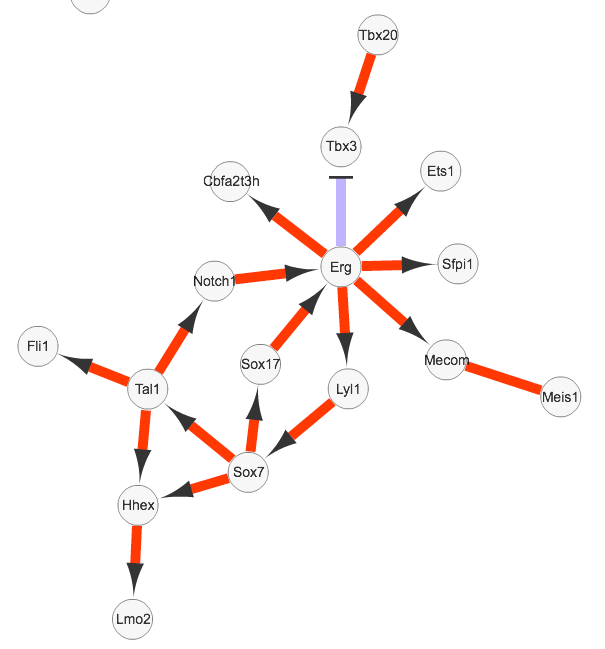
\includegraphics[width=\linewidth]{results/filtre4SFG33genes2}
\caption{Population des cellules 4SFG (à partir des FT). On peut remarquer le rôle central du FT Erg.}
\label{fig:pop4SFG}
\end{figure*}

\begin{figure*}[ht]
\centering
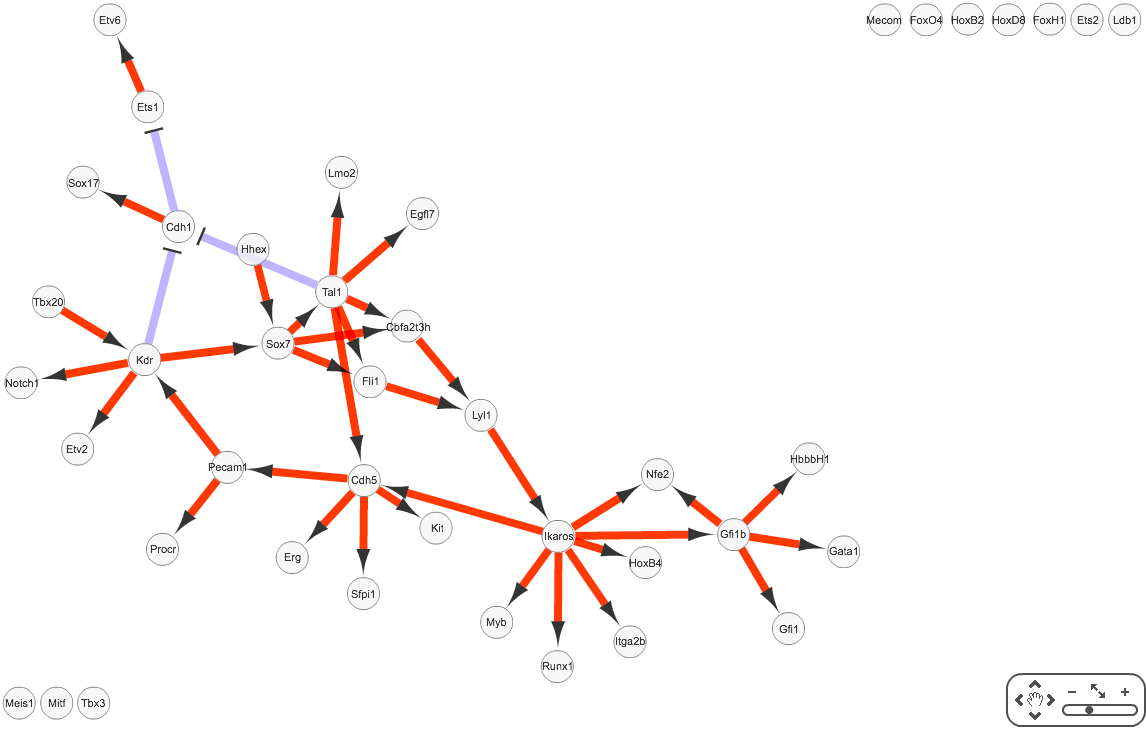
\includegraphics[width=\linewidth]{results/filtreNP}
\caption{Population des cellules NP (à partir des 42 gènes). Notons l'inhibition de l'inhibiteur de Ets1 et activateur de Sox17 (Cdh1). Rôle central de Kdr, Tal1, Cdh5, Ikaros, Gfi1b}
\label{fig:popNP}
\end{figure*}

\begin{figure*}[ht]
\centering
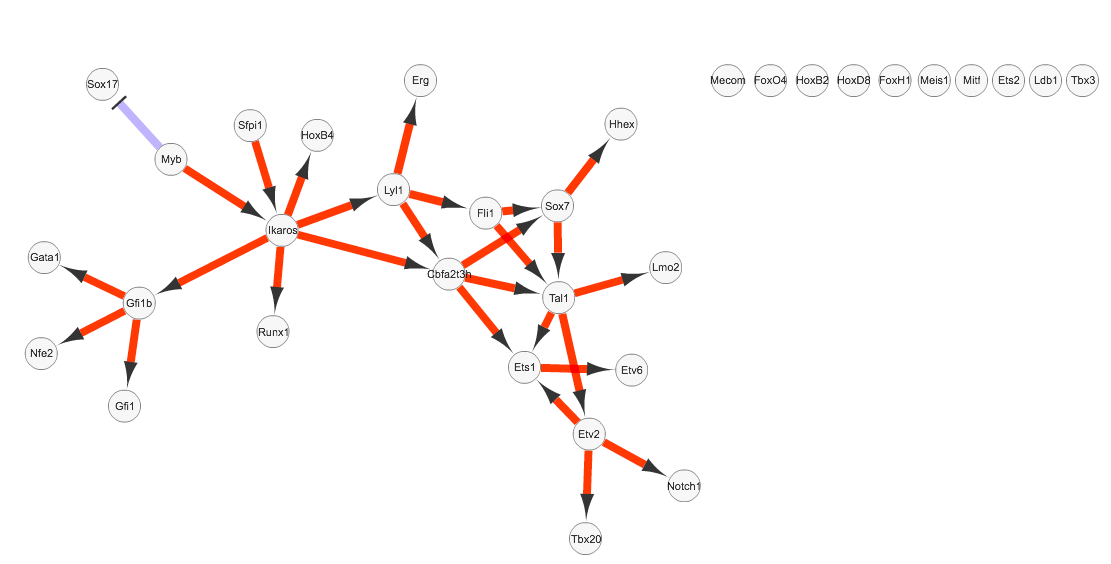
\includegraphics[width=\linewidth]{results/filtreNP33genes2}
\caption{Population des cellules NP (à partir des 33 gènes) : perte des interactions liées aux gènes marqueurs Cdh1 et Cdh5 par rapport au graphe avec 42 gènes, fondamentales pour la différenciation - le graphique précédent permet donc une visualisation plus précise des interactions au stade NP}
\label{fig:popNP33}
\end{figure*}


\begin{figure*}[ht]
\centering
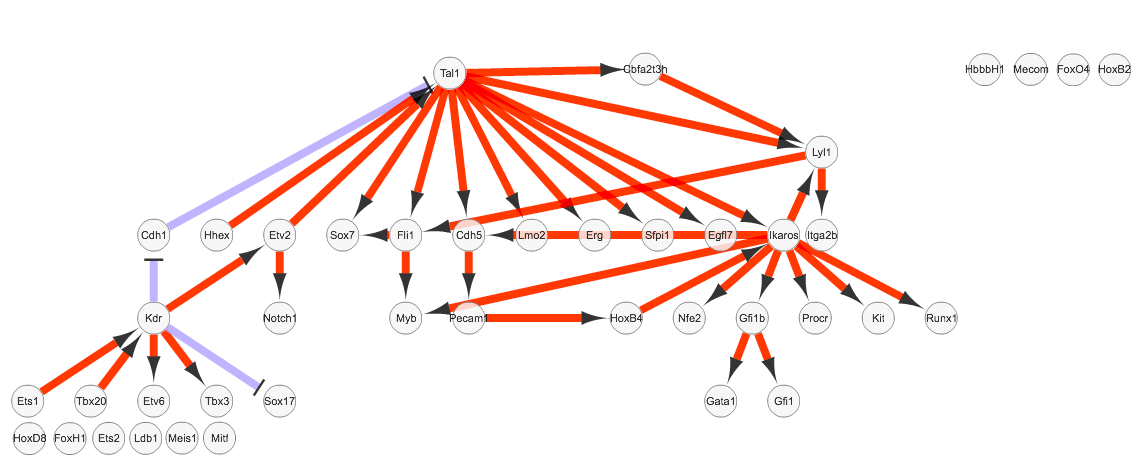
\includegraphics[width=\linewidth]{results/filtrePS2}
\caption{Population des cellules PS (à partir des 42 gènes). Kdr agit comme régulateur négatif du gène marqueur Cdh1 qui lui-même agit négativement sur Tal1. Rôle central de Kdr, Tal1 et Ikaros. Inhibition de Sox17.}
\label{fig:popPS}
\end{figure*}

\begin{figure*}
\centering
\includegraphics[scale=0.9]{results/filtreHF2}
\caption{Population des cellules HF (à partir des 42 gènes). Notons l'inhibition de Kdr par Cdh1 et de Gfi1b par Sox17. Rôle central de Tal1, Cdh1, Fli1, Lyl1, Ikaros.}
\label{fig:popHF}
\end{figure*}


\begin{figure*}[ht]
\centering
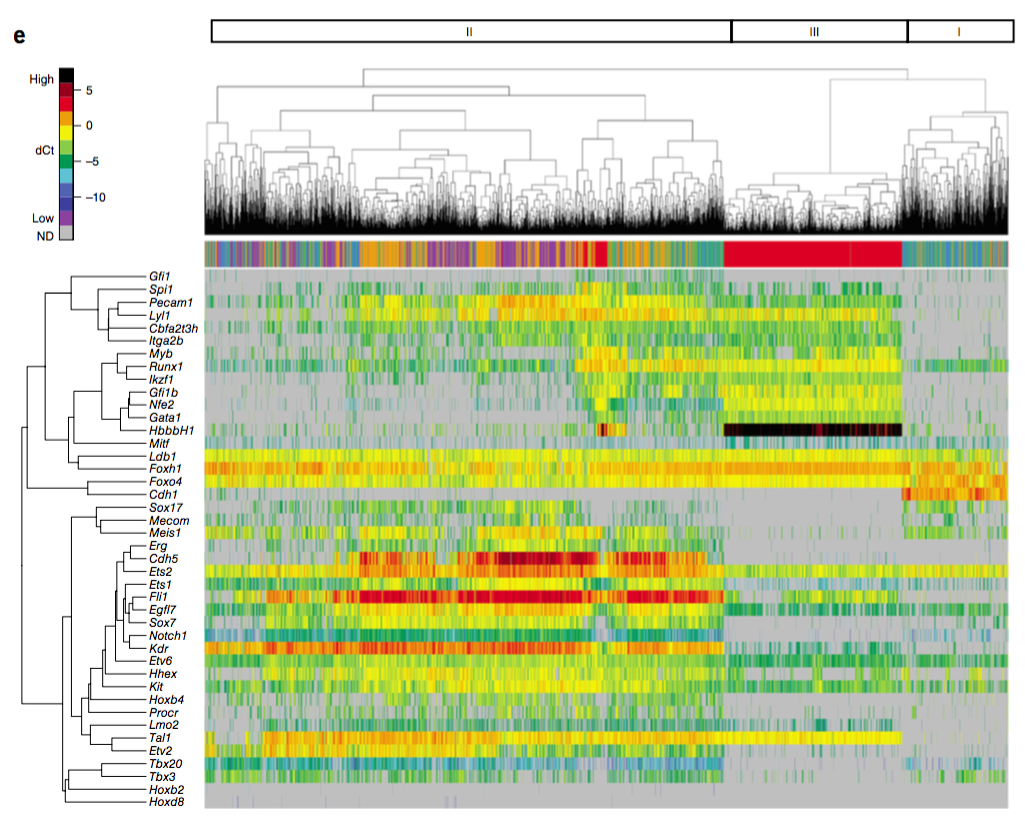
\includegraphics[width=\linewidth]{images/article2}
\caption{Résultats du clustering hierarchique non supervisé issus de \textit{Moignard et al.} à partir de l'analyse par \textit{single cell}. On peut observer le niveau d'expression pour chaque gène dans toutes les cellules. Les colonnes représentent les cellules et les lignes les gènes. Les couleurs correspondent au stade embryonnaire d'où chaque cellule a été extraite.}
\label{fig:article2}
\end{figure*}


%\begin{figure*}[ht]
%\centering
%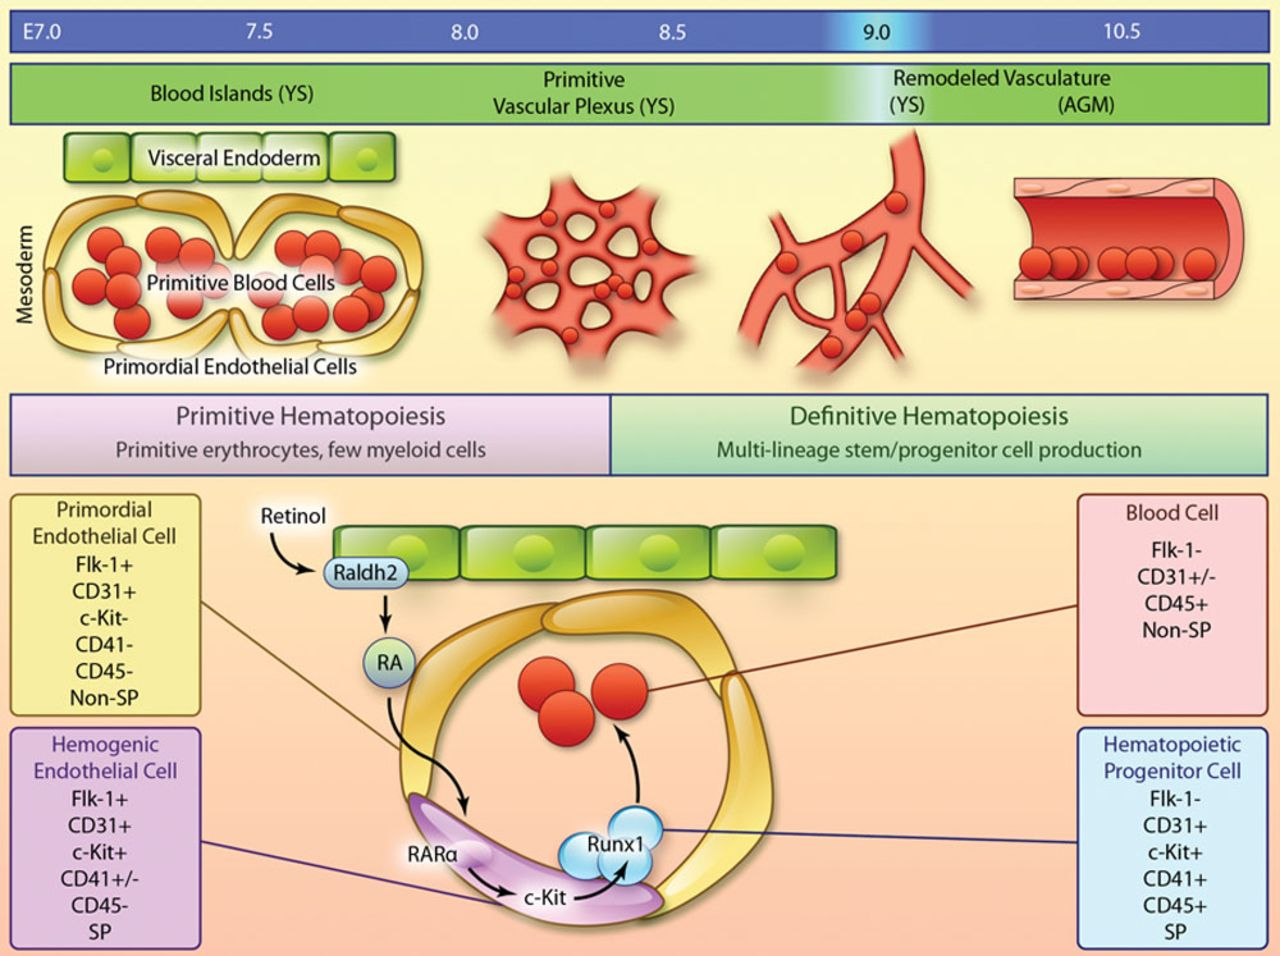
\includegraphics[width=\linewidth]{images/synthese}
%\caption{Parallèle entre l'hématopoïèse et la formation des vaisseaux sanguins à des stades du développement précoce embryonnaire (vertébrés)\href{http://circres.ahajournals.org/content/112/9/1272}{\cite{Marcelo}}}
%\label{fig:synthese}
%\end{figure*}


\begin{figure*}[ht]
\centering
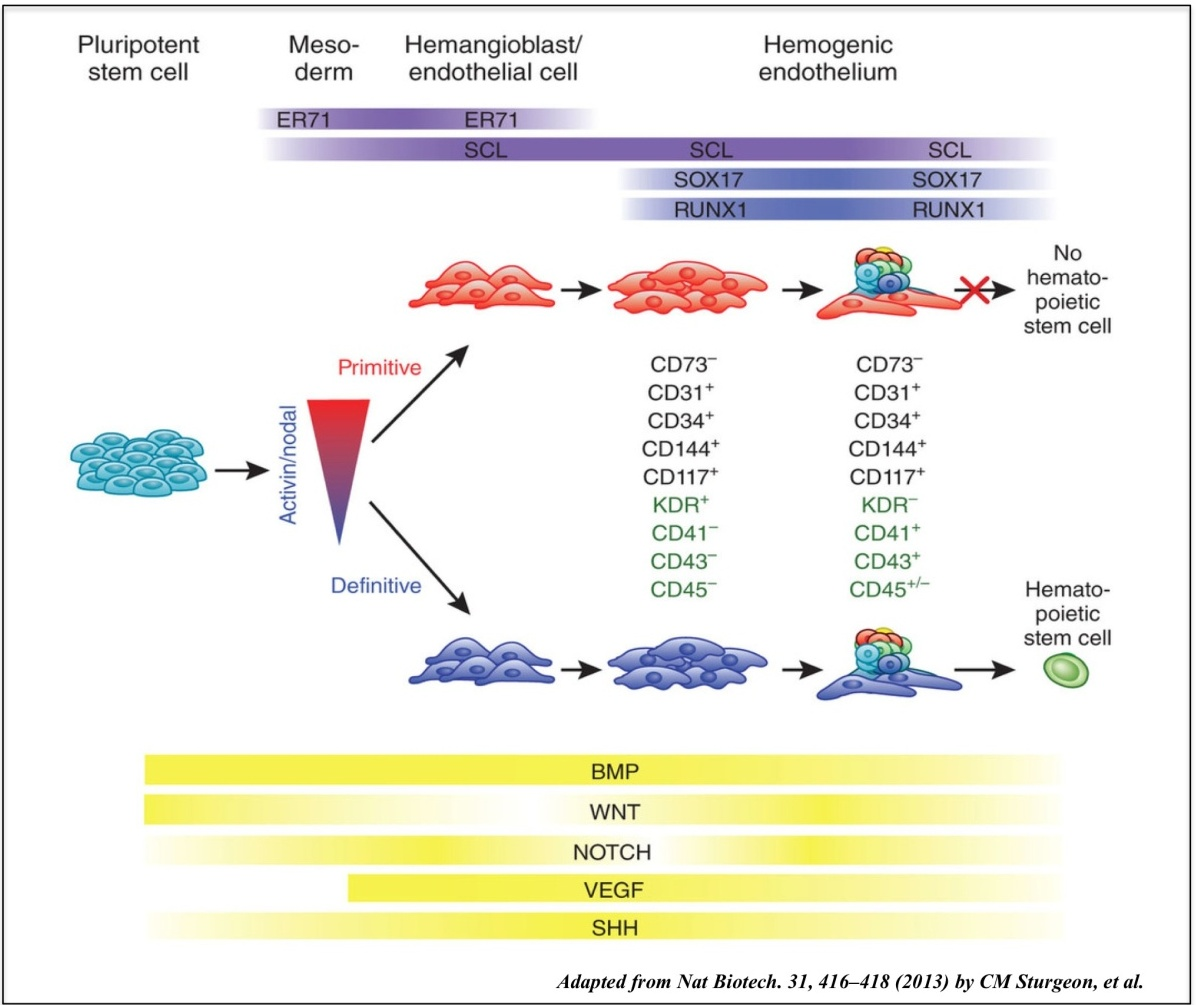
\includegraphics[width=\linewidth]{images/syntheseSuper}
\caption{Développement de l'hémangioblaste (précurseur commun des cellules endothéliales et hématopoïétiques) et de l'épithélium hémogénique à partir de cellules pluripotentes\href{http://cdn.intechopen.com/pdfs-wm/46823.pdf}{\cite{Chen}}}
\label{fig:syntheseSuper}
\end{figure*}


\begin{figure*}[ht]
\centering
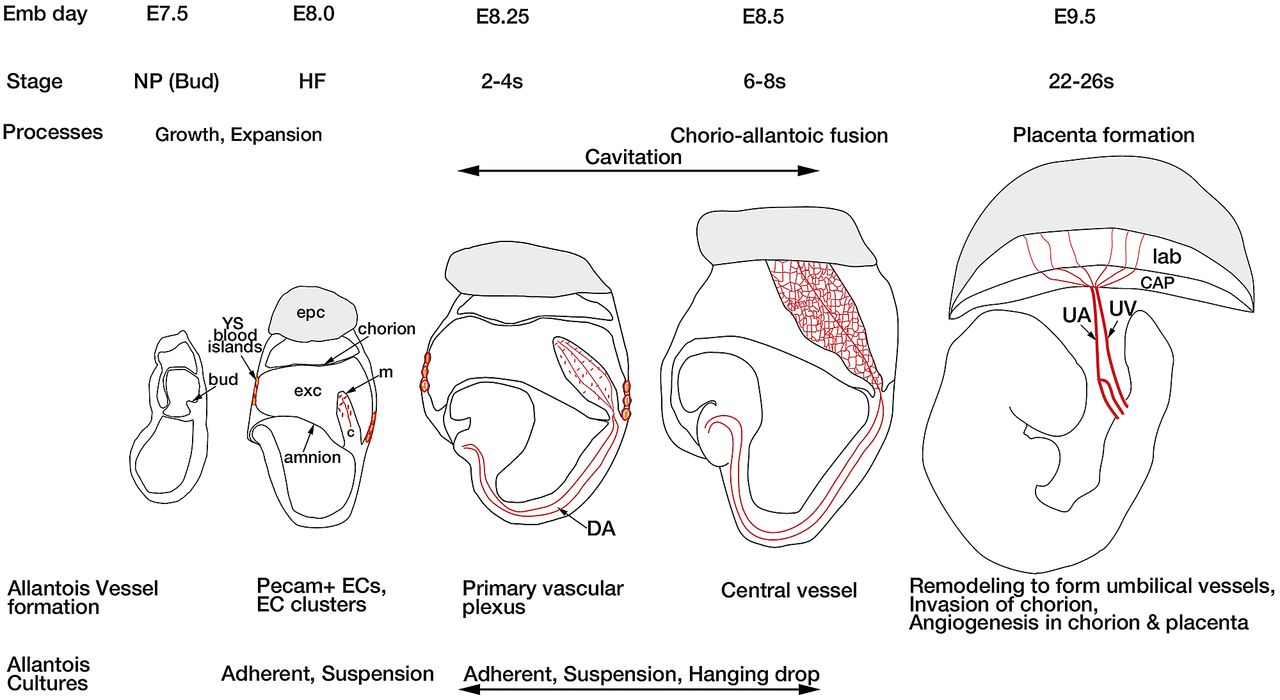
\includegraphics[width=\linewidth]{images/devpt}
\caption{Détails du développement précoce de \textit{Mus musculus}\href{http://www.ipubli.inserm.fr/handle/10608/6217}{\cite{Gaudin}} du stade E7 à E11.5, dans le compartiment extra-embryonnaire (en rouge) et intra-embryonnaire (en jaune). En encart figurent les sites impliqués dans la génération des CSH, c’est-à-dire l’aorte et sa partie ventrale (et les artères omphalomésentérique (OA) et ombilicale (UA)). AGM : aorte-gonades-mésonephros ; FF : foie fœtal ; P-Sp : splanchnopleure para-aortique ; Sp : splanchnopleure ; SV : sac vitellin}
\label{fig:devpt}
\end{figure*}

%\begin{figure}[ht]
%\centering
%\includegraphics[width=\linewidth]{images/ikarosNotchGata}
%\caption{ikaros - Notch - Gata}
%\label{fig:ikarosNotchGata}
%\end{figure}


 % http://embomolmed.embopress.org/content/7/11/1388


%\section*{Annexes}

%\begin{figure*}[ht]
%\centering
%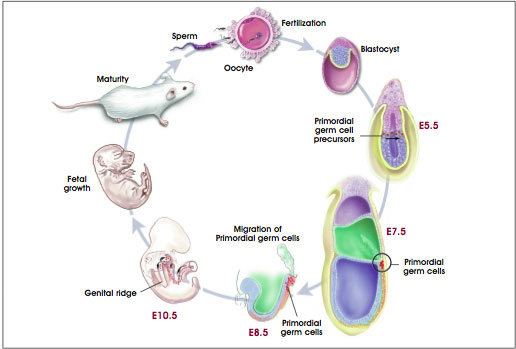
\includegraphics[width=\linewidth]{images/devptCycle}
%\caption{Cycle de développement de \textit{Mus musculus}}
% https://stemcells.nih.gov/info/2001report/appendixA.htm
%\label{fig:devptCycle}
%\end{figure*}



%\addcontentsline{toc}{section}{Annexes}
%
%\subsection*{Matériel additionnel} 
%\addcontentsline{toc}{subsection}{Matériel additionnel}
%\subsubsection{Filtres}
%\subsubsection{Fonction de score}

%\begin{figure}[ht]\centering
%\includegraphics[width=\linewidth]{images/poidsScoring}
%\caption{Poids utilisés pour les fonctions de score (utilisés dans RosettaDock\cite{rosettaDOCK}, pour le scoring de haute définition)}
%\label{fig:poidsScoring}
%\end{figure}



%\subsection*{Chronologie du docking}
%\addcontentsline{toc}{subsection}{Chronologie du docking}
%
%\subsection*{Outils de docking}
%\addcontentsline{toc}{subsection}{Outils de docking}


%----------------------------------------------------------------------------------------
%	REFERENCE LIST
%----------------------------------------------------------------------------------------

%----------------------------------------------------------------------------------------

\end{document}






%Articles de réf\cite{Pedotti}
%ref\cite{Rajkannan}
%ref\cite{Sela-Culang}
%ref\cite{Kuroda}
%ref\cite{Krawczyk}
%ref\cite{Abhinandan}
%ref\cite{Gabb}
%\cite{proABC}

%\url{http://www.wikibooks.org}


% Reference to Figure \ref{fig:results}.

%\begin{description}
%\item[Word] Definition
%\item[Concept] Explanation
%\item[Idea] Text
%\end{description}


%\begin{figure*}[ht]\centering % Using \begin{figure*} makes the figure take up the entire width of the page
%\includegraphics[width=\linewidth]{view}
%\caption{Wide Picture}
%\label{fig:view}
%\end{figure*}
%
%\lipsum[4] % Dummy text
%
%\begin{equation}
%\cos^3 \theta =\frac{1}{4}\cos\theta+\frac{3}{4}\cos 3\theta
%\label{eq:refname2}
%\end{equation}
%
%\lipsum[5] % Dummy text
%
%\begin{enumerate}[noitemsep] % [noitemsep] removes whitespace between the items for a compact look
%\item First item in a list
%\item Second item in a list
%\item Third item in a list
%\end{enumerate}
%
%\subsection{Subsection}
%
%\lipsum[6] % Dummy text
%
%\paragraph{Paragraph} \lipsum[7] % Dummy text
%\paragraph{Paragraph} \lipsum[8] % Dummy text
%
%\subsection{Subsection}
%
%\lipsum[9] % Dummy text
%
%\begin{figure}[ht]\centering
%\includegraphics[width=\linewidth]{results}
%\caption{In-text Picture}
%\label{fig:results}
%\end{figure}
%

%\begin{table}[hbt]
%\caption{Table of Grades}
%\centering
%\begin{tabular}{llr}
%\toprule
%\multicolumn{2}{c}{Name} \\
%\cmidrule(r){1-2}
%First name & Last Name & Grade \\
%\midrule
%John & Doe & $7.5$ \\
%Richard & Miles & $2$ \\
%\bottomrule
%\end{tabular}
%\label{tab:label}
%\end{table}

%\footnote{And some mathematics $\cos\pi=-1$ and $\alpha$ in the text.}.
